\newpage
\subsection{Mechanical Design} \label{Mechanical_Design}
\label{sec:mechanical-design}

\subsubsection{Structure}
\label{sec:4.4.1}
The experiment itself has only two components that are placed inside the gondola. Firstly, the electronics box and then the gimbal on which the telescope is mounted. We require the gimbal to be placed at the edge of the gondola so that the telescope setup is stowed during launch and descent, but still capable of being deployed and performing its required range of motion for observing astronomical targets outside of the gondola.

\begin{figure}[H]
   \begin{minipage}[t]{0.6\textwidth}   
	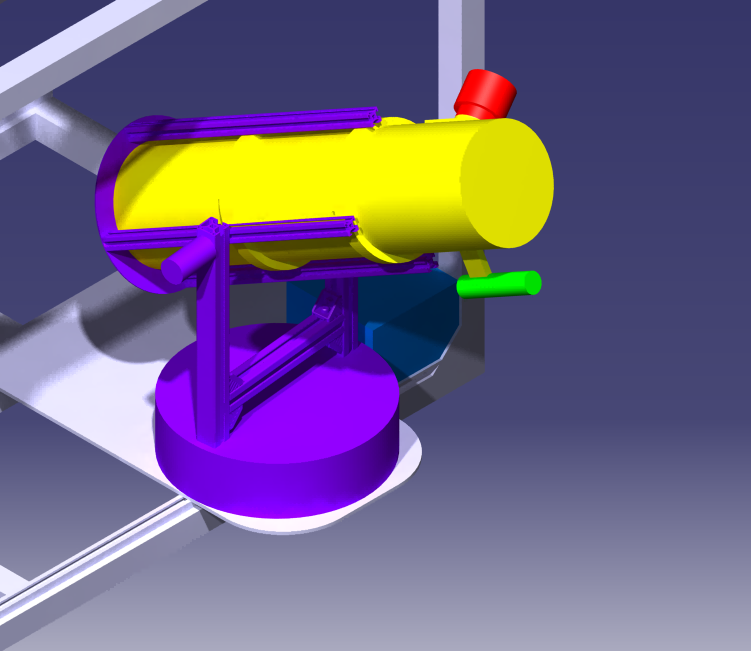
\includegraphics[scale=1.4]{4-experiment-design/img/mechanical/Assembly_v3iso.png}
	\caption{Overview of experiment structure. Image updated}
	\label{fig::mechanical::IsoView1}
	\end{minipage}
	\hfill
	\begin{minipage}[t]{0.4\textwidth}
	\vspace{-5cm}	
	\begin{tabular}{c | c}
	Color & Component \\ \hline
	Yellow & Telescope\\
	Purple & Gimbal\\
	Red & NIR Camera\\
	Green & Guiding camera\\
	Blue & Electronics box\\	
	\end{tabular}	
\end{minipage}		 
\end{figure}


\subsubsection{Electronics box}
\label{sec:4.4.2}


The electronics box has a dimension 10x10x10 cm which is placed directly inside the gondola, \hl{see figure {\ref{fig::mechanical::ebox}}} . It is estimated to weigh 1.5 kg. The box is made of aluminium side plates with a thick layer of styrofoam placed on the inside of the aluminium plates which protects the electronics. The box has rubber cushion feet that acts as a shock absorber and also thermal insulator from the gondola.

\begin{figure}[H]
	\centering 
	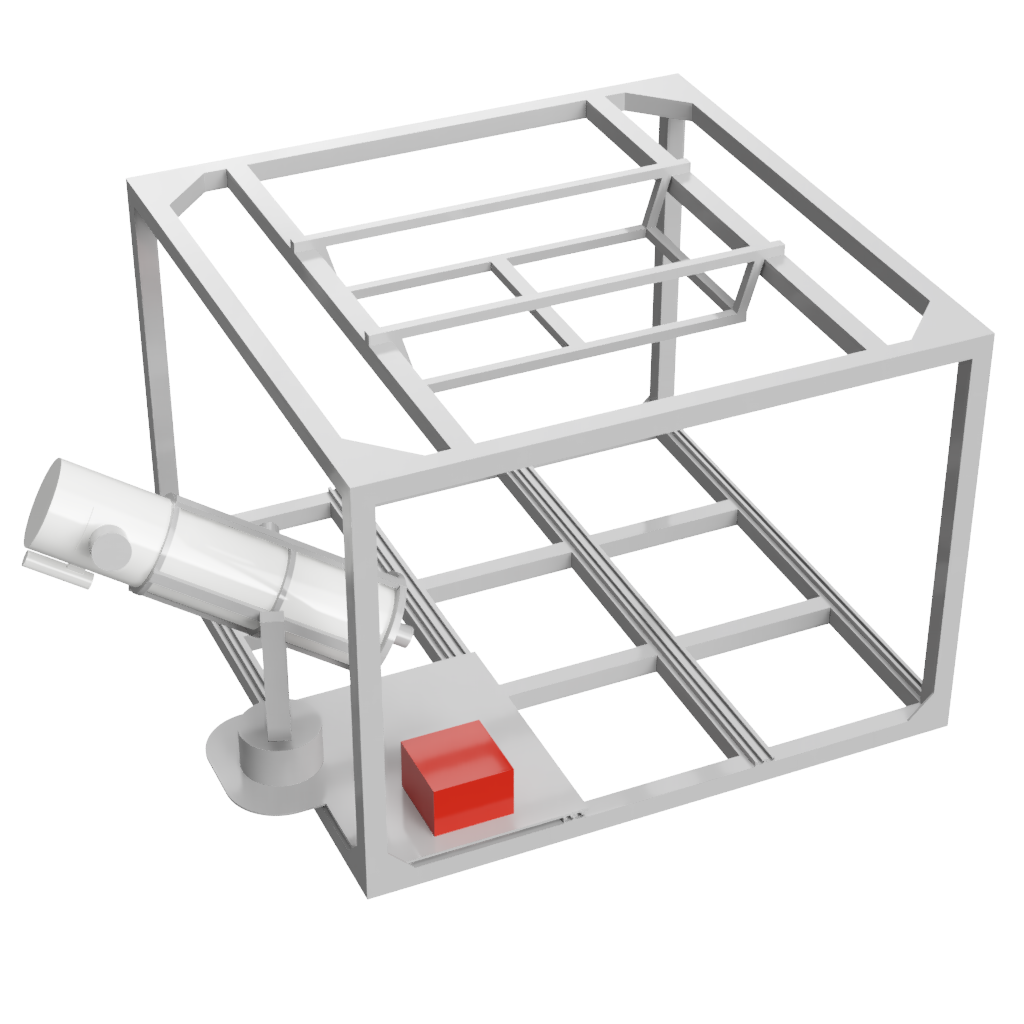
\includegraphics[scale=0.4]{4-experiment-design/img/mechanical/ebox.png}
	\caption{\hl{Electronics box placement[new figure].}}
	\label{fig::mechanical::ebox}
\end{figure}


\subsubsection{Gimbal}
\label {sec:4.4.3}

The gimbal structure is made from aluminium extrusions with standard fastener brackets, steel rods and sheet aluminium. It uses three geared DC motors, 6 radial bearings in standard press-fit mounts and two open needle roller thrust bearings. Refer to \ref{sec:mech_drawings} for detail sketches. 

Testing will be conducted to evaluate the structures' rigidity. The mass budget allows for stiffening the structure by adding steel plates and steel wire braces as needed. Critical parts, i. e. the glide bearing surfaces, can be milled using a two axis CNC machine. 

The motors provide a peak torque of 0.3 N/m. Assumning the mass of the telescope and gimbal assembly to be about 6 kg with all mass concentrated at the ends of the telescope the moment of inertia around the vertical (Z) axis is on the order of 2.2 kg/m\textsuperscript{2}. Neglecting bearing friction this gives a maximum angular acceleration of about 7.5\textdegree/s\textsuperscript{2}. All other axes will have lower moments of inertia. The roll axis will have signifficant friction which is difficult to predict. If necessary the glide bearings can be replaced by three radial bearings each, but this is not prefferred due to complexity and precision requirements. 

All three axles are driven by 8 mm D-slotted steel shafts. Torque is transferred to moving parts using steel clamping brackets with setscrews. All axes except the vertical are directly connected to the motors using 5 to 8 mm shaft adapter collars with set screws. The vertical axis is driven by means of a 1:1 gear so that the motor can be mounted on the top side of the mounting plate. The vertical axis has the longest shaft at about 100 mm. Using standard methods for torsion estimation it was found that this steel shaft will twist 0.05\textdegree when the motor is providing the maximum rated torque. 

The azimuth axis is supported laterally by two radial bearings. The lower bearing is attached to the base plate and the upper bearing on an aluminium plate that is elevated by 10 standoffs in a 5-fold star pattern to ensure rigidity. Because the axis is mostly vertical and the telescope center of mass is directly on the axis the side forces on the bearings are expected to be neglible. The radial bearings are offloaded axially by means of a needle roller thrust bearing on the upper plate, that presses against the steel shaft clamp on the horisontal member of the gimbal cradle. Refer to illustration \ref{img:az_sketch} in Appendix C. The thrust bearing will experience a static load less than 70 N. The entire assembly is retained upwards by the main shaft gear which rests on the lower bearing. 

The elevation axis is divided in two sections to accomodate the telescope tube. Each side is supported by two radial bearings. To allow for thermal expansion only the undriven side of the elevation assembly is retained by means of shaft collars, which means that any motion will be transferred to the motor output shaft which has some axial play by design. See image \ref{img:el_sketch} in Appendix C. The entire axis can be moved by sliding the shaft clamping plates in the slots of the axial aluminium extrusions on the roll cage assembly, thus moving the telescope center of mass to the desired position. 

For the roll axis the entire telescope is supported by two glide bearing surfaces. The glide bearing structures are machined from  aluminium and split along the axial aluminium extrusions to simplify attachment and removal of the telescope. The  two halves of each glide bearing ring are dimensioned such that they do not rest directly on the axial aluminium extrusions. This facilitates some adjustment using the mounting screws. The roll cage is stiffened by four axial rods made from either steel, aluminium or carbon fiber (tentative). The gliding surfaces are clad with teflon bushing material to minimize friction. To avoid pinching and buckling the glide surfaces have breaks at regular intervals that allows for some thermal expansion. See image \ref{img:el_sketch} in Appendix C. 

The third axis motor is mounted on an aluminim plate behind the telescope and elevated on an adapter plate to accomodate the encoder and coupling collar, see illustration \ref{img:roll_sketch} in Appendix C. The rear of the telescope is clamped in a three-point vice, akin to a centering chuck on a lathe. The vice is made from aluminium plate and angle brackets, with set screws that allows precise alignment of the telescope. The vice is coupled to the main shaft through a steel clamping collar with a set screw. the axial force from the telescope is unloaded from the motor by means of a thrust bearing between the clamping collar and the motor mounting plate. No force is expected to act in the forward direction on the telescope. Therefore the entire assembly is only retained in the forward direction by the motor shaft and coupling. 

\begin{figure}[h]
	\centering
	\begin{minipage}[t]{0.4\linewidth}
		\centering
		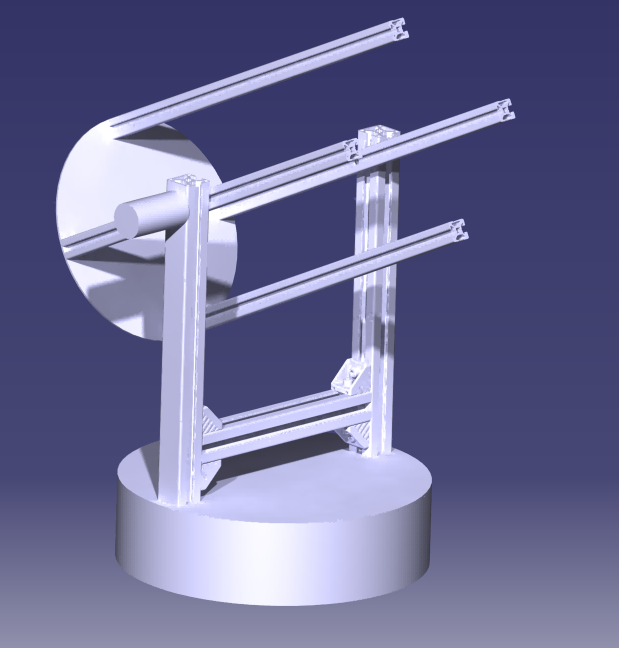
\includegraphics[width=\linewidth]{4-experiment-design/img/mechanical/Aluminium_Gimbal1.png}
		\caption{Aluminium Gimbal proposed design}
		\label{fig::mechanical::AlGim}
	\end{minipage}
	%\hfill
	\hspace{0.1\linewidth}
	\begin{minipage}[t]{0.4\linewidth}
		\centering
		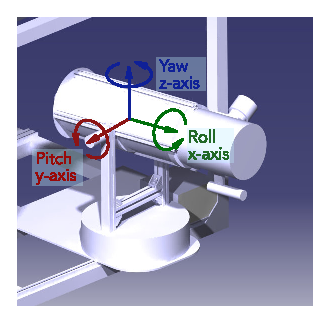
\includegraphics[width=\linewidth]{4-experiment-design/img/software/Yaw_Pitch_Roll.eps}
	\caption{Yaw, Pitch and Roll angles of the gimbal}
	\label{fig::software::Yaw_Pitch_Roll}
	\end{minipage}

\end{figure}





\subsubsection{Fixing interface}
\label {sec:4.4.5}
The mounting plate will be fixed to the gondola using a simple aluminium frame attached to the rails of the Gondola. The gimbal along with the fixing points will first be tested with Finite Element Analysis (FEA) in order to ensure that the whole structure can withstand the loads indicated in the BEXUS manual.
